\documentclass[fleqn]{beamer}
\beamertemplatenavigationsymbolsempty

\usepackage[T1]{fontenc}
\usepackage[utf8]{inputenc}

\usepackage{amsmath,amssymb}
\usepackage{graphicx}
\usepackage{mathptmx}
\usepackage{subcaption}
\usepackage{amsthm}
\usepackage{tikz}
%\usepackage[colorlinks=true,naturalnames=true,plainpages=false,pdfpagelabels=true]{hyperref}
\usetikzlibrary{patterns,decorations.pathmorphing,positioning, arrows, chains}

\usepackage[backend=biber, sorting=none]{biblatex}
\addbibresource{uni.bib}

\setbeamertemplate{endpage}{%
    \begin{frame}
        \centering
        \Large \emph{To be continued\ldots}

        \vspace{1cm}

        \centering
        \Large \emph{Thank You!}
    \end{frame}
}

\AtEndDocument{\usebeamertemplate{endpage}}

% vertical separator macro
\newcommand{\vsep}{
  \column{0.0\textwidth}
    \begin{tikzpicture}
      \draw[very thick,black!10] (0,0) -- (0,7.3);
    \end{tikzpicture}
}
\setlength{\mathindent}{0pt}

% Beamer theme
\usetheme{UniVienna}
\usefonttheme[onlysmall]{structurebold}
\mode<presentation>
\setbeamercovered{transparent=10}

\title
{Seminar Complex Network Analysis}
\subtitle{Project Progress}
\author[Popović Milutin]
{Popović Milutin}
\date{5. May 2021}

\begin{document}
    \begin{frame}
        \titlepage
    \end{frame}

    \begin{frame}
        \frametitle{Reminder}
        \centering
        \textbf{Python Package Dependency Network}
        \vspace{1cm}
        \begin{columns}[T]
            \column{0.4\textwidth}
            \column{0.4\textwidth}
        \end{columns}
    \end{frame}

    \begin{frame}
        \frametitle{Reminder}
        \centering
        \textbf{Python Package Dependency Network}
        \vspace{1cm}
        \begin{columns}[T]
            \column{0.4\textwidth}
        \begin{align*}
            \text{Nodes}\ &\to\  \text{Repositories}\\
            \text{Edges}\ &\to\ \text{Requirements}(Imoprts)
        \end{align*}
            \column{0.4\textwidth}
        \end{columns}
    \end{frame}

    \begin{frame}
        \frametitle{Reminder}
        \centering
        \textbf{Python Package Dependency Network}
        \vspace{1cm}
        \begin{columns}[T]
            \column{0.4\textwidth}
        \begin{align*}
            \text{Nodes}\ &\to\  \text{Repositories}\\
            \text{Edges}\ &\to\ \text{Requirements}(Imoprts)
        \end{align*}
            \column{0.4\textwidth}
        \begin{block}{\centering Directed Graph}
            \centering \texttt{scipy $\to$ numpy}\\
            \centering \texttt{scipy $\not\gets$ numpy}
        \end{block}
        \end{columns}
    \end{frame}

    \begin{frame}
        \frametitle{Revisiting the Data}
        \begin{itemize}
            \item[$\to$] Python Package Index (PyPi) gives release
                information for every version of a package
        \end{itemize}
        \vspace{6cm}
    \end{frame}

    \begin{frame}
        \frametitle{Revisiting the Data}
        \begin{itemize}
            \item[$\to$] Python Package Index (PyPi) gives release
                information for every version of a package
        \end{itemize}
        \centering \textbf{requests=="0.10.0"}
        \begin{figure}
            \centering
            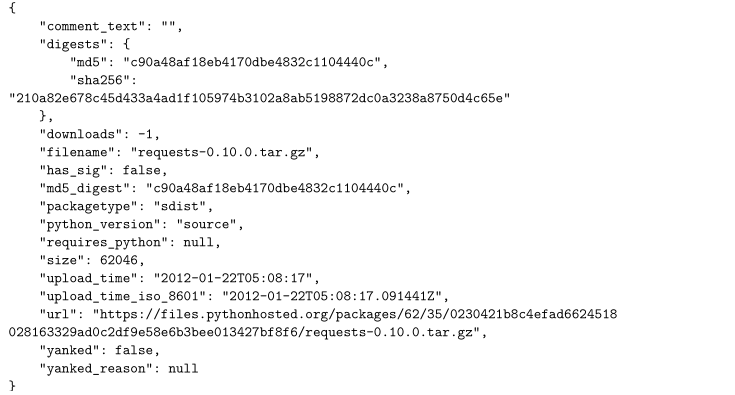
\includegraphics[width=0.8\textwidth]
                             {./pics/json.png}
        \end{figure}
    \end{frame}

    \begin{frame}
        \frametitle{Revisiting the Data}
        \begin{itemize}
            \item[$\to$] Python Package Index (PyPi) gives release
                information for every version of a package
        \end{itemize}
        \centering \textbf{requests=="0.10.0"}
        \begin{figure}
            \centering
            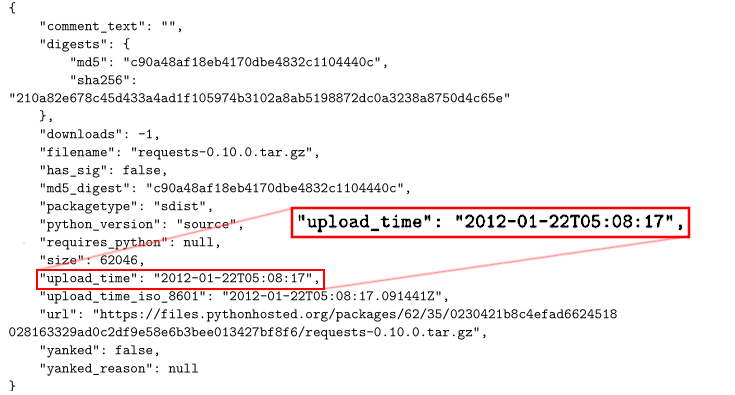
\includegraphics[width=0.8\textwidth]
                             {./pics/select_json.png}
        \end{figure}
    \end{frame}

    \begin{frame}
        \frametitle{Revisiting The Data}
        \begin{columns}[T]
            \column{0.4\textwidth}
        \begin{align*}
            \to &\;\;\text{sort nodes \& links based on release date}\\
                &\Rightarrow\; \text{Time dependent directed network}
        \end{align*}
        \end{columns}
    \end{frame}

    \begin{frame}
        \frametitle{Dealing with Time dependent Graphs}
            \centering $\to$\;\; Child-Class of \texttt{nx.DiGraph}\\
            \vspace{4.2cm}
    \end{frame}

    \begin{frame}
        \frametitle{Dealing with Time dependent Graphs}
            \centering $\to$\;\; Child-Class of \texttt{nx.DiGraph}\\
            \centering $\to$\;\; Every edge has a time-stamp e.g.\\
            \vspace{0.5cm}
            \centering \hspace{0.5cm} \texttt{scipy} $\rightarrow$
            \texttt{numpy} at $t = \text{2016-4}$
            \vspace{3cm}
    \end{frame}

    \begin{frame}
        \frametitle{Dealing with Time dependent Graphs}
            \centering $\to$\;\; Child-Class of \texttt{nx.DiGraph}\\
            \centering $\to$\;\; Every edge has a time-stamp e.g.\\
            \vspace{0.5cm}
            \centering \hspace{0.5cm} \texttt{scipy} $\rightarrow$
            \texttt{numpy} at $t = \text{2016-4}$
            \vspace{1cm}

            \centering \texttt{class TDiGraph(nx.DiGraph)}
        \begin{columns}[T]
            \column{0.45\textwidth}
        \begin{block}{\centering Class Method: forward}
            \centering add edges with time-stamp $t$\\
            \centering set $t = t + 1$
        \end{block}
            \column{0.45\textwidth}
        \end{columns}
    \end{frame}

    \begin{frame}
        \frametitle{Dealing with Time dependent Graphs}
            \centering $\to$\;\; Child-Class of \texttt{nx.DiGraph}\\
            \centering $\to$\;\; Every edge has a time-stamp e.g.\\
            \vspace{0.5cm}
            \centering \hspace{0.5cm} \texttt{scipy} $\rightarrow$
            \texttt{numpy} at $t = \text{2016-4}$
            \vspace{1cm}

            \centering \texttt{class TDiGraph(nx.DiGraph)}
        \begin{columns}[T]
            \column{0.45\textwidth}
        \begin{block}{\centering Class Method: forward}
            \centering add edges with time-stamp $t$\\
            \centering set $t = t + 1$
        \end{block}
            \column{0.45\textwidth}
        \begin{block}{\centering Class Method: backward }
            \centering remove edges with time-stamp $t$\\
            \centering set $t = t - 1$
        \end{block}
        \end{columns}
    \end{frame}

    \begin{frame}
        \frametitle{Traveling Back in Time}
        \begin{figure}[htpb]
            \centering
            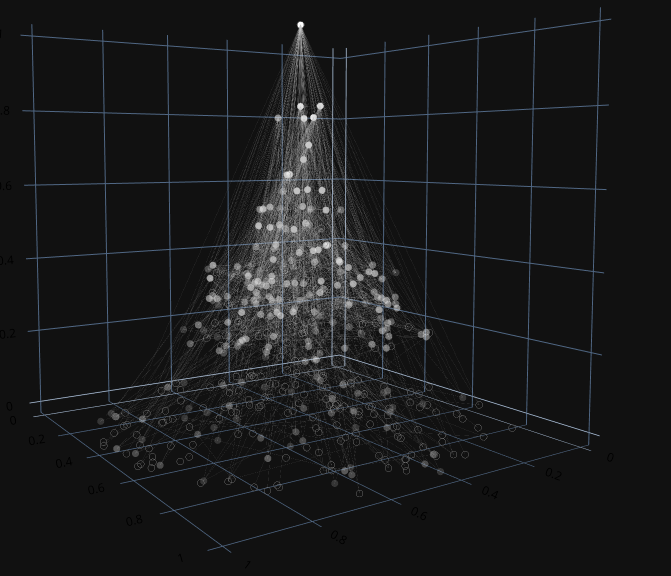
\includegraphics[width=0.45\textwidth]{./pics/plot_2015.png}
            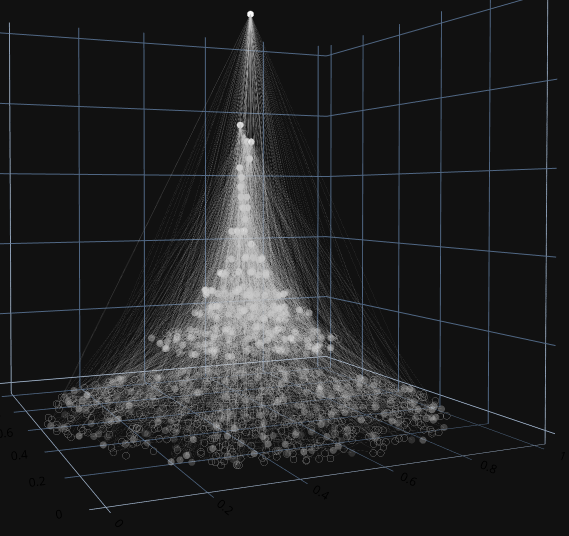
\includegraphics[width=0.45\textwidth]{./pics/plot_sqrt.png}
            \caption{Left: Graph from 2015, Right: Graph from 2022}
        \end{figure}
    \end{frame}

    \begin{frame}
        \frametitle{Observations}
        \begin{figure}[htpb]
            \centering
            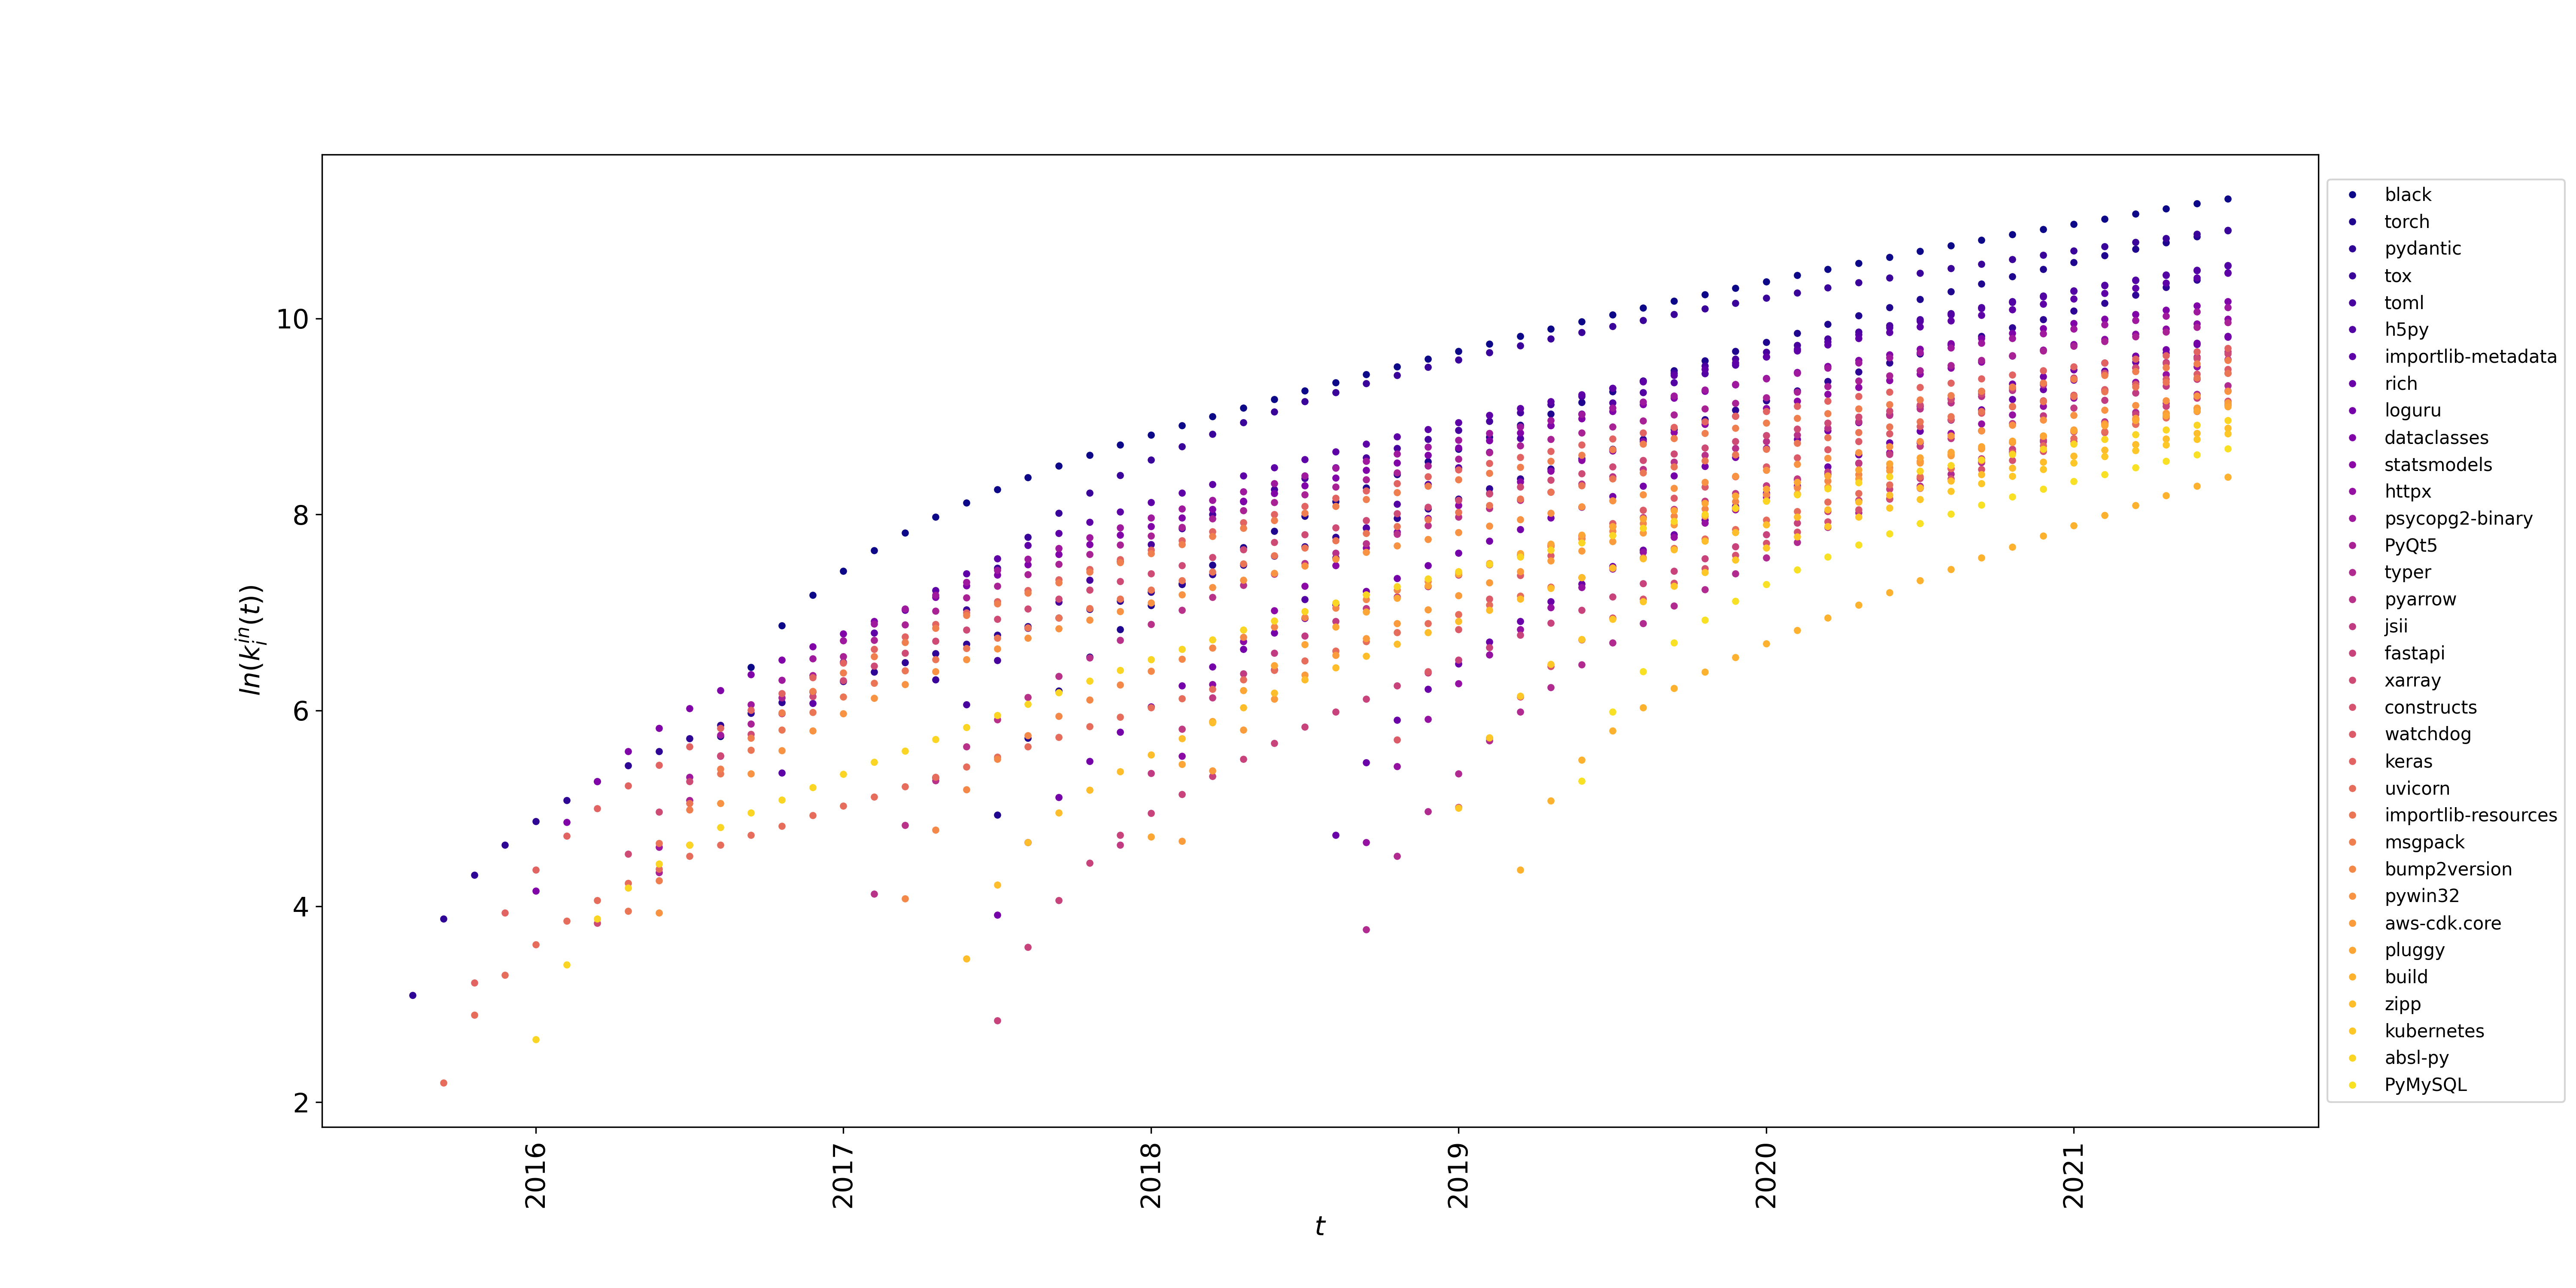
\includegraphics[width=0.8\textwidth]{./pics/edge_growth.png}
            \caption{Growth-Exponent $\beta_i$ of the top nodes}
        \end{figure}
    \end{frame}

    \begin{frame}
        \frametitle{Observations}
        \begin{figure}[htpb]
            \centering
            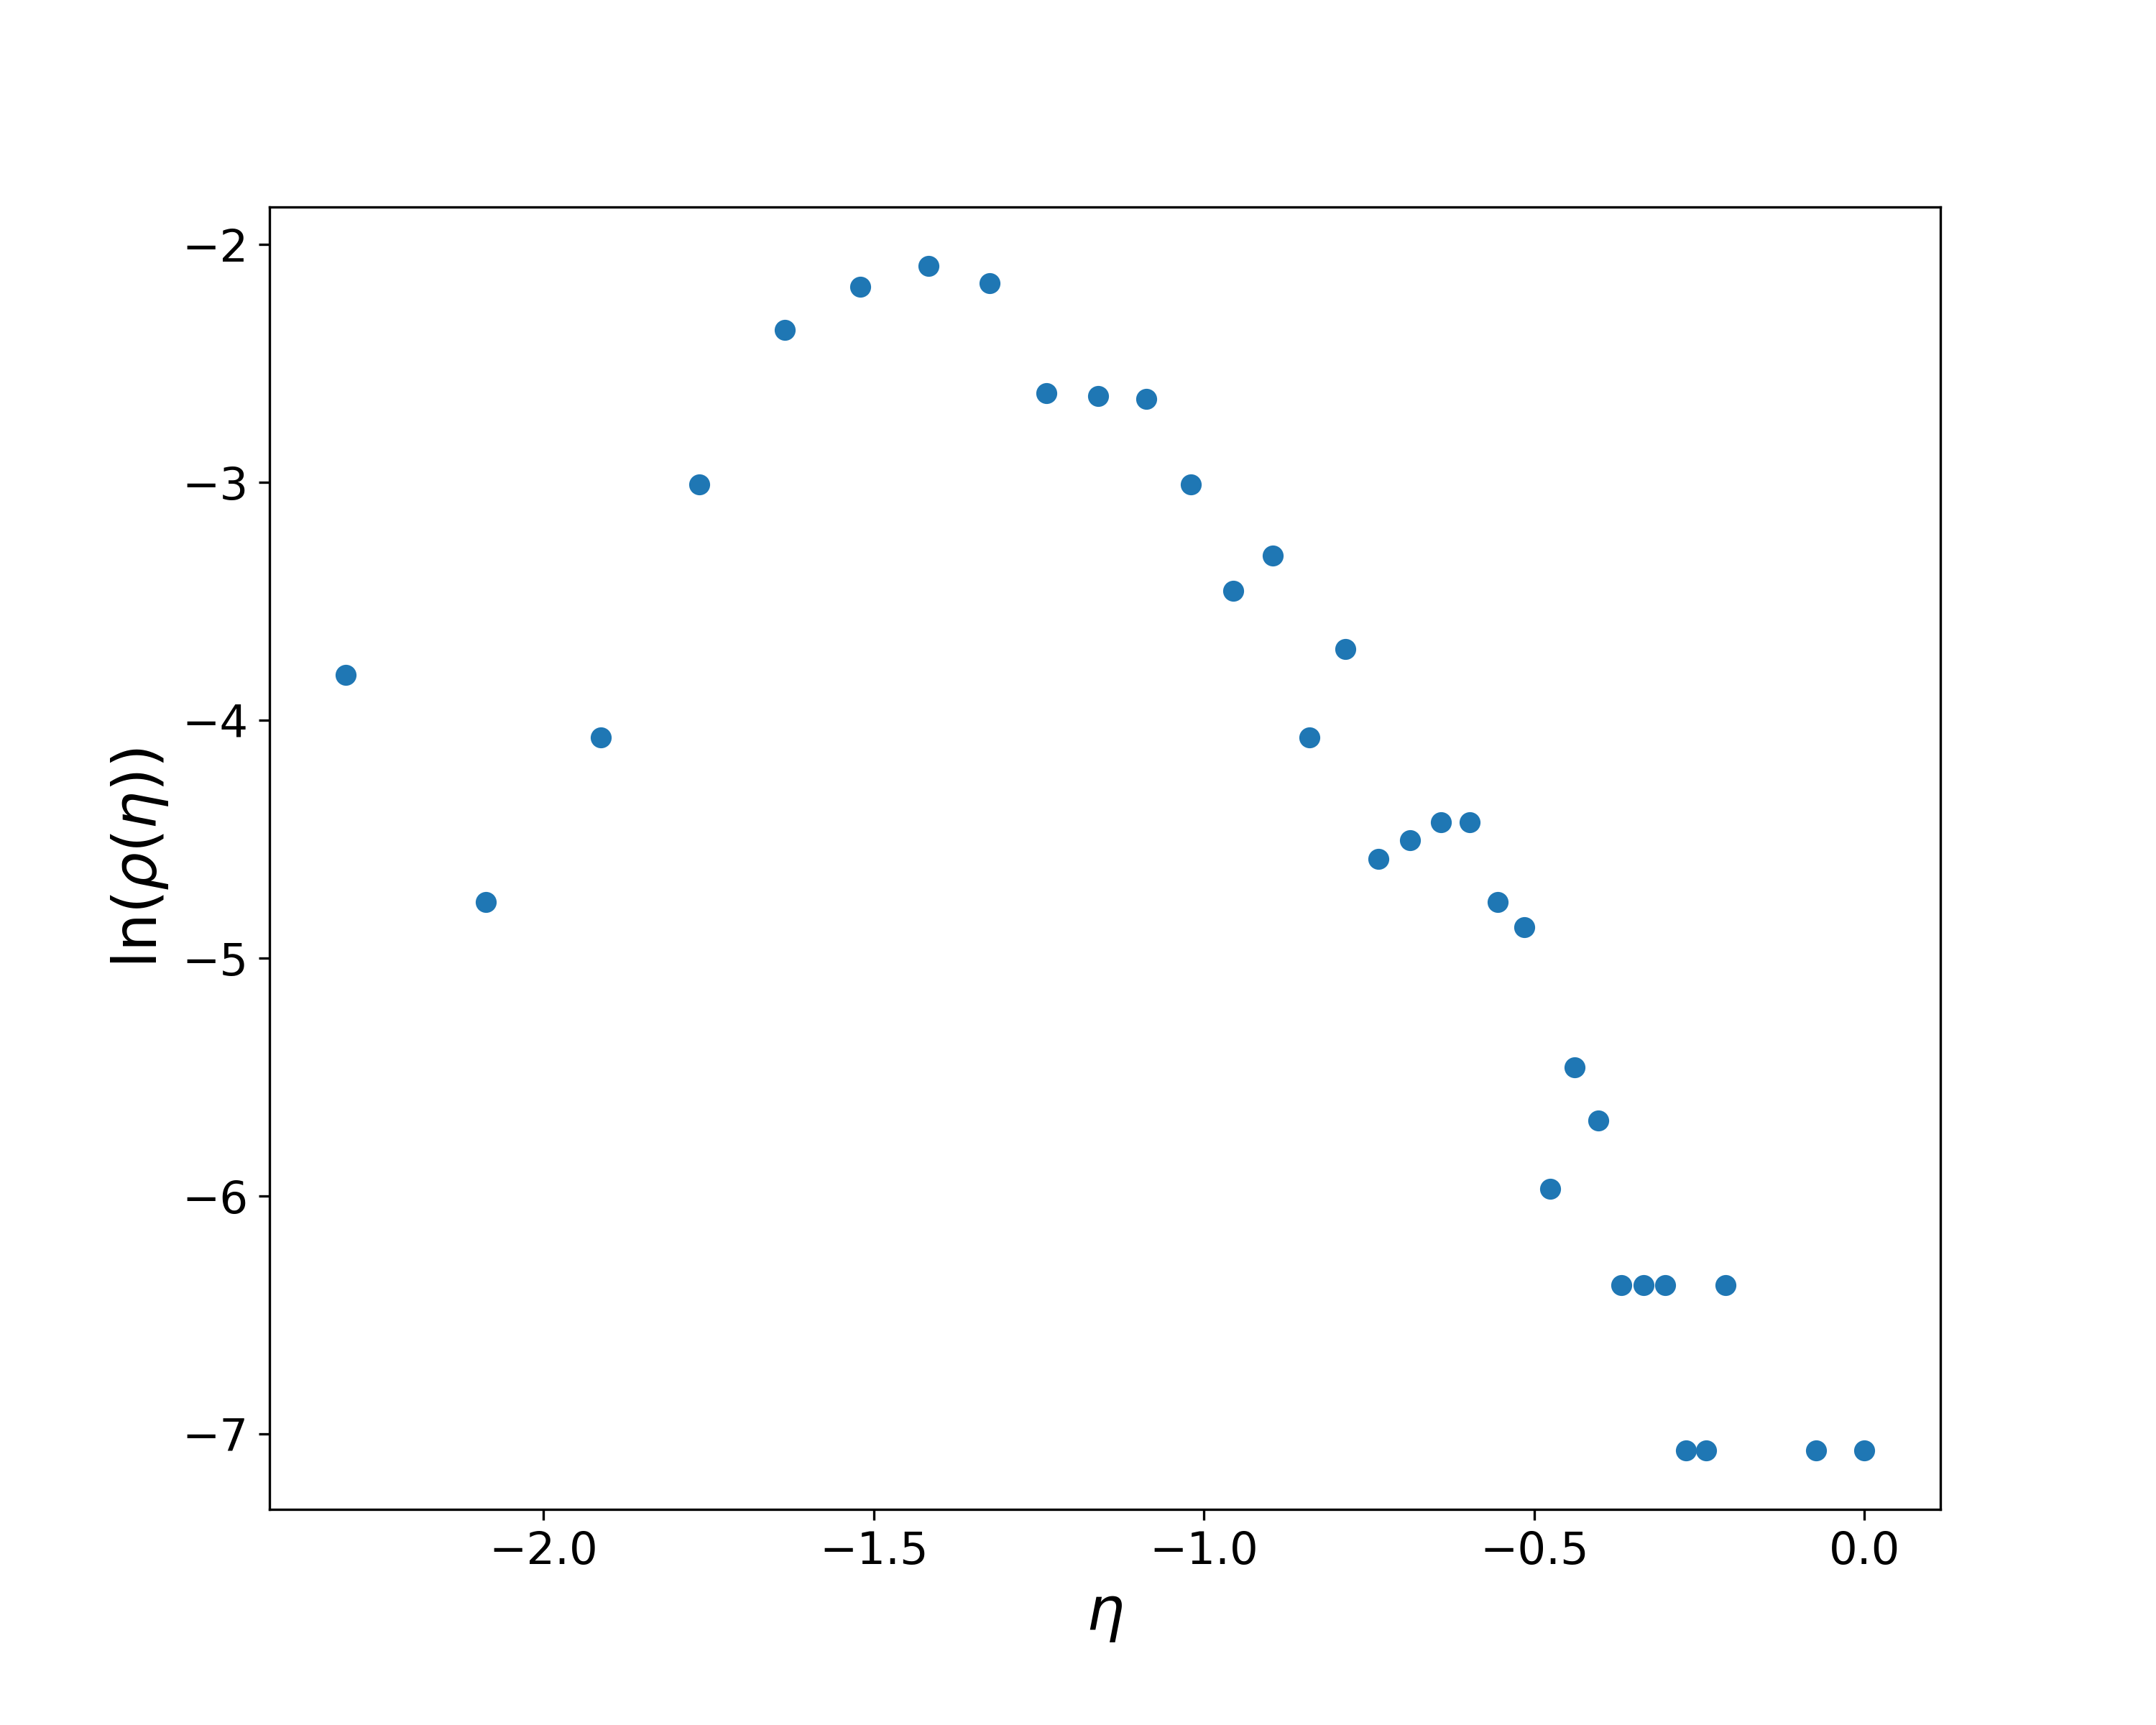
\includegraphics[width=0.8\textwidth]{./pics/fitness.png}
            \caption{Distribution of the node fitness $\rho(\eta)$}
        \end{figure}
    \end{frame}

    \begin{frame}
        \frametitle{Visualizing the Network: Layout}
        \centering \textbf{Idea: ``Light-Ray'' Layout}
    \end{frame}

    \begin{frame}
        \frametitle{Visualizing the Network: Layout}
        \centering \textbf{Idea: ``Light-Ray'' Layout}
        \begin{itemize}
            \item[$\to$] separate nodes based on their degree
        \end{itemize}
    \end{frame}

    \begin{frame}
        \frametitle{Visualizing the Network: Layout}
        \centering \textbf{Idea: ``Light-Ray'' Layout}
        \begin{itemize}
            \item[$\to$] separate nodes based on their degree
            \item[$\to$] place them each uniformly on a circle/disks
                distance
        \end{itemize}
    \end{frame}

    \begin{frame}
        \frametitle{Visualizing the Network: Layout}
        \centering \textbf{Idea: ``Light-Ray'' Layout}
        \begin{itemize}
            \item[$\to$] separate nodes based on their degree
            \item[$\to$] place them each uniformly on a circle/disks
            \item[$\to$] stack the disks, based on a function representing their
                distance
        \end{itemize}
    \end{frame}

    \begin{frame}
        \frametitle{Visualizing the Network: Layout}
        \begin{figure}[htpb]
            \centering
            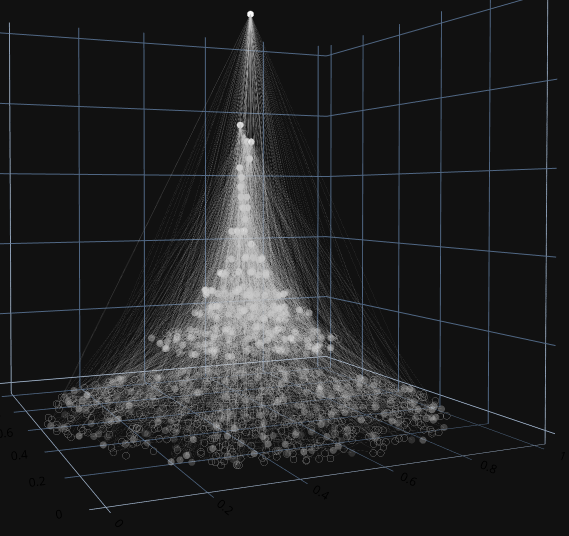
\includegraphics[width=0.7\textwidth]{./pics/plot_sqrt.png}
        \end{figure}
    \end{frame}

    \begin{frame}
        \frametitle{Visualizing the Network: Layout}
        \begin{figure}[htpb]
            \centering
            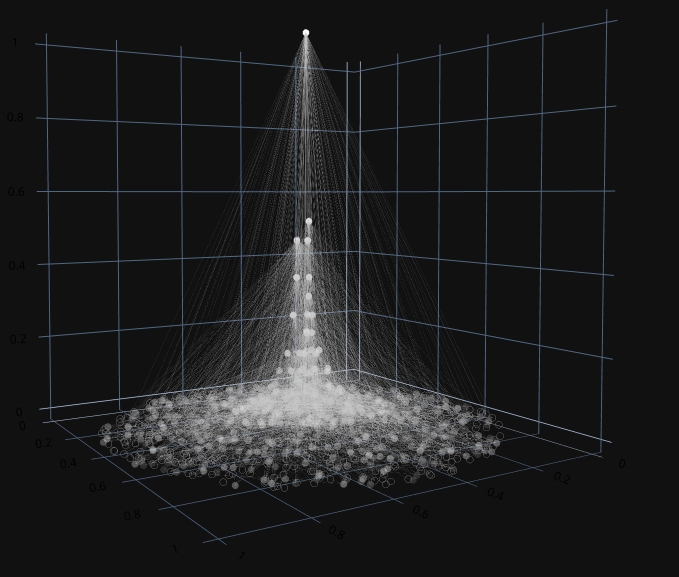
\includegraphics[width=0.7\textwidth]{./pics/plot_lin.png}
        \end{figure}
    \end{frame}

    \begin{frame}
        \frametitle{Visualizing the Network: Layout}
        \begin{figure}[htpb]
            \centering
            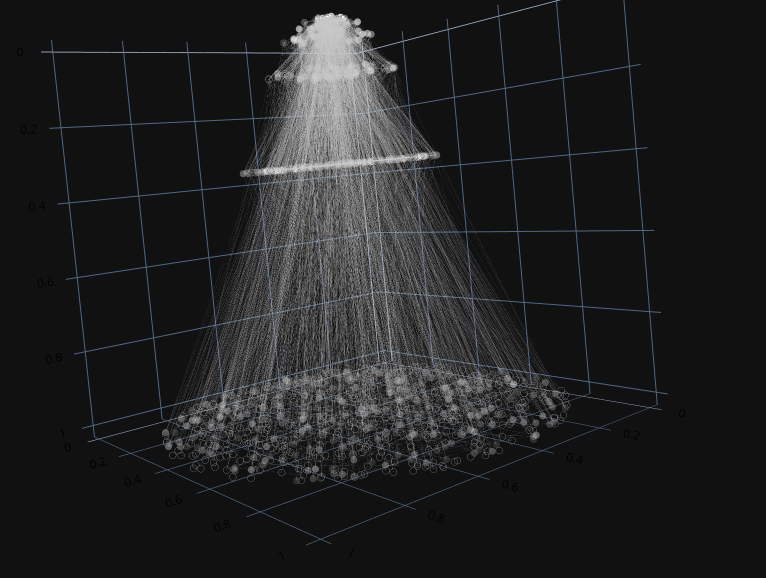
\includegraphics[width=0.7\textwidth]{./pics/plot_exp.png}
        \end{figure}
    \end{frame}

    \begin{frame}
        \frametitle{Visualizing the Network: Layout}
        \begin{figure}[htpb]
            \centering
            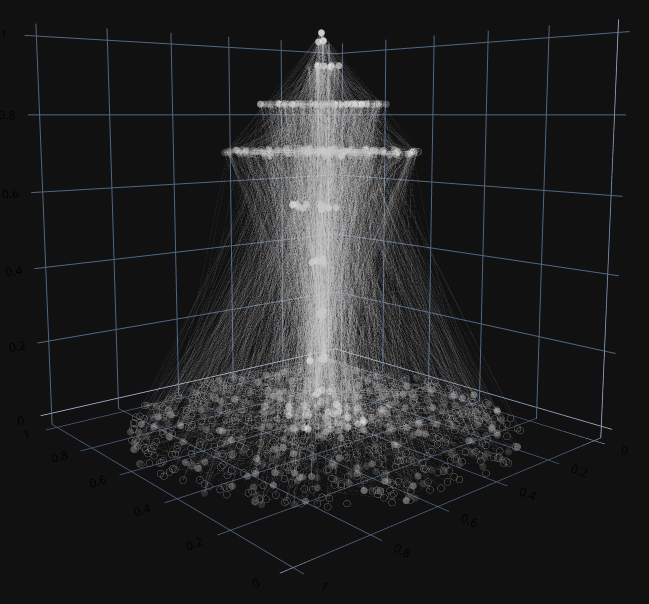
\includegraphics[width=0.7\textwidth]{./pics/plot_sin2.png}
        \end{figure}
    \end{frame}

    \begin{frame}{Bibliography}
        \nocite{barabasi}
        \nocite{pypi}
        \printbibliography
    \end{frame}
\end{document}

